\section{The Central Divergence: Saturation of the Published Safety Term}

Shen's composite score combines acuity, fill factor, ghost safety and
coverage into one number, with ghost safety entering as a smooth,
sigmoid-shaped membership function rather than a hard cutoff:
\begin{equation}
g = \frac{s f' / L}{c_{\text{tot}}}, \qquad \mu_g = \sigma\big(2(1-g)\big), \qquad g_{\max}=1
\end{equation}

\subsection{What Happens When This Is Applied to This Project's Own Data}
Computed directly, for all 8501 candidate rows in this project's dataset:
\begin{center}
\begin{tabular}{lr}
\toprule
Quantity & Value \\
\midrule
$g$, minimum & 33.9 \\
$g$, maximum & 2423.7 \\
$g$, mean & 418.9 \\
$g$, median & 271.7 \\
Fraction of rows with $\mu_g < 10^{-10}$ & \textbf{100.0\%} \\
Fraction with $\mu_g$ at exact floating-point zero & 35.3\% \\
\bottomrule
\end{tabular}
\end{center}

\findbox{Every single candidate in this project's tested design space has
$g \gg 1$. The sigmoid membership $\mu_g$ is numerically zero, or
indistinguishable from zero, for 100\% of rows --- not most, not typically,
all of them. The published ghost-safety term contributes nothing to the
ranking on this project's actual candidates, for either safe or unsafe
designs.}

\begin{figure}[h]
\centering
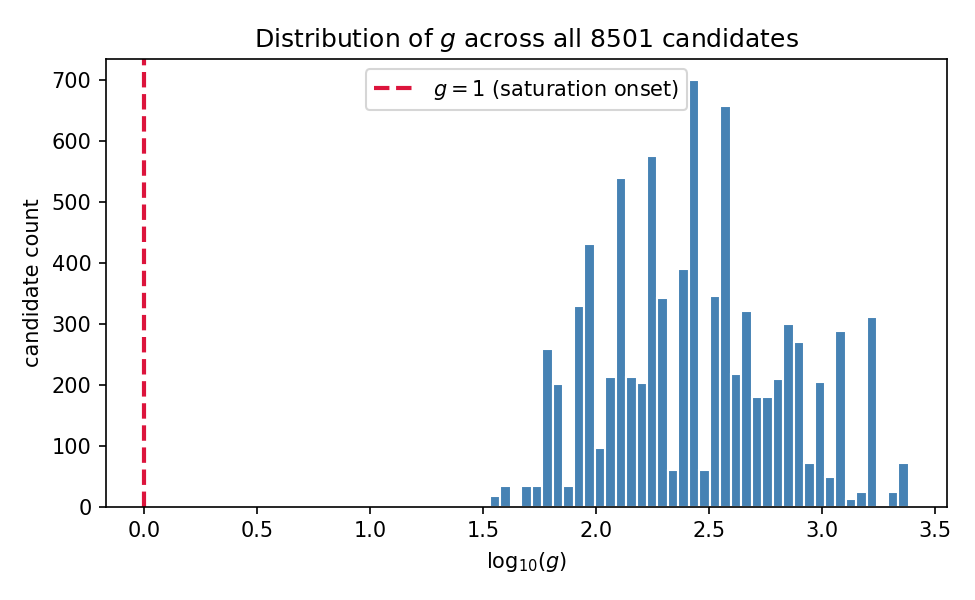
\includegraphics[width=0.75\textwidth]{compare_pdf_figs/fig_g_distribution.png}
\caption{Distribution of $g$ across all 8501 candidates. The entire
distribution sits far to the right of $g=1$, the point where $\mu_g$ begins
to saturate.}
\end{figure}

\begin{figure}[h]
\centering
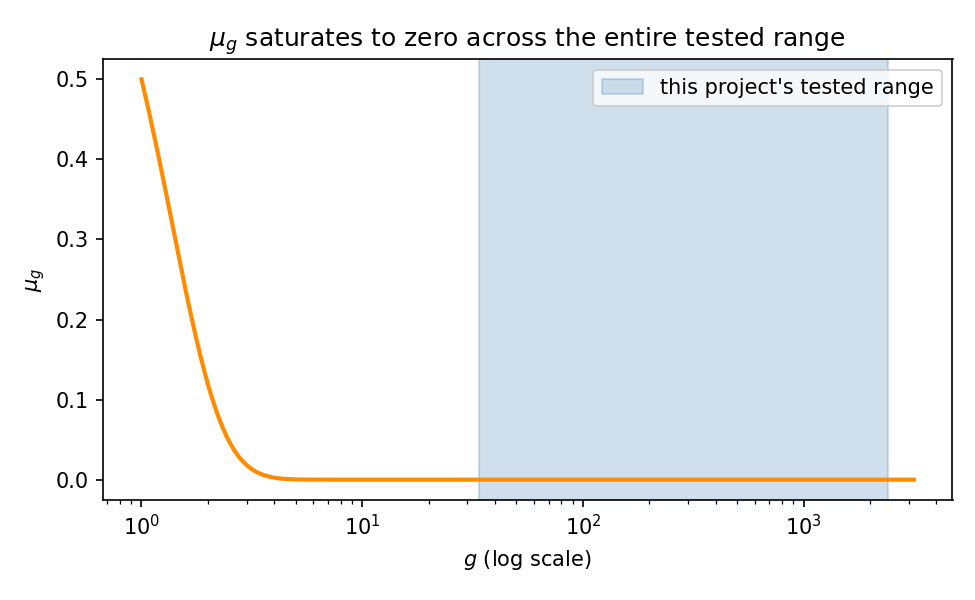
\includegraphics[width=0.75\textwidth]{compare_pdf_figs/fig_mu_g_saturation.png}
\caption{The $\mu_g$ sigmoid curve with this project's entire tested $g$
range shaded. The whole range sits in the flat, saturated tail.}
\end{figure}

\newpage
